The CMS RPC upgrade for Phase-2~\cite{muon_tdr} compreehends \textbf{(1) the replacement of a the current Link System}, which connects the Front-End Boards (FEBs) to the trigger processors, by a new one, redesigned from scratch and \textbf{(2) the extension of the pseudorapidity coverage of the RPC system}, by adding new chamber from $|\eta| = 1.9$ up to 2.4, namely stations RE3/1 and RE4/1. Those new chamber will be assembled with a Improved Resistive Plate Chambers (iRPC) technology, with does the readout of signals, in both ends of the strip. The timing difference per hit and strip, is used by the iRPC Front-End to estimate the spatial position of the hit in the longitudinal direction. The current RPC chambers can only read the transverse hit position.

\begin{wrapfigure}{r}{0.6\textwidth}
    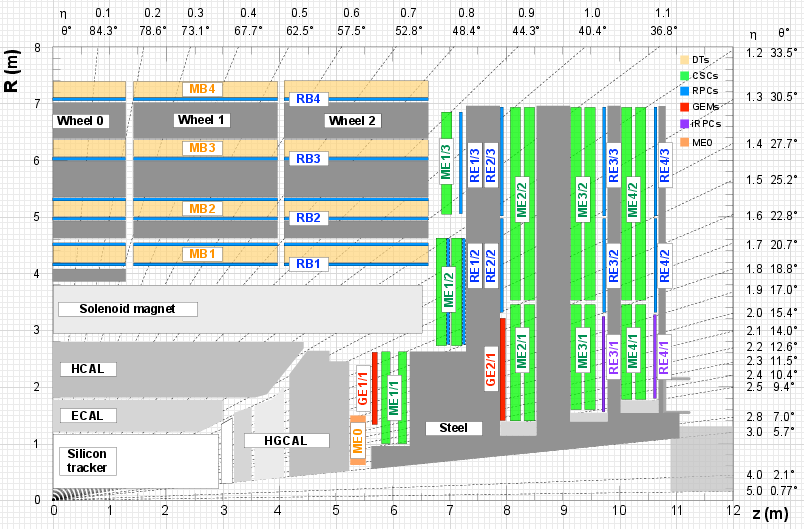
\includegraphics[width=0.6\textwidth]{uioposter-images/cms_muon}
    \caption{CMS Muon system for the Phase-2 Upgrade.}
    \label{cms_muon_upgrade}
\end{wrapfigure}


Both upgrades are important in order to cope with expected high rate of the HL-LHC scenario, in which a Inst. Luminosity of $5 \times 10^{34}$ $cm^{-2}s^{-1}$ would provide a bckground ate of up to 700 $Hz/cm^2$ (already including a safety factor of 3). Also, the upgrades woiuld enhance the redundancy of the CMS Muon System, resolve ambiguities in the endcap triggering and allow improvements of the RPC system to Trigger and reconstruction. Figure 1 presents a quadrant of the CMS Muon system, showing Drift Tubes (DT) chambers in yellow, RPCs in light blue, and Cathode Strip Chambers (CSCs) in green. The locations of new forward muon detectors for the HL-LHC project are indicated in red for Gas Electron Multiplier (GEM) stations (ME0, GE1/1, and GE2/1) and violet for improved RPC stations (RE3/1 and RE4/1).

